\section{Simple correspondence analysis}\label{sec:ca-simple}
\ixon{correspondence analysis!two-way tables}
\subsection{Notation and terminology}\label{sec:ca-notation}
Because \CA\ grew up in so many homes, the notation, formulae
and terms used to describe the method vary considerably.
The notation used here generally follows \citet{Greenacre:84,Greenacre:97},
as does the documentation in the \STUGref{19}{The CORRESP Procedure}.

The descriptions here employ the following matrix and vector definitions:
\begin{itemize}
\item $\mat{N} = \{ n_{ij} \}$ is the $I \times J$ contingency table
with row and column totals $n_{i+}$ and $n_{+j}$, respectively.
The grand total $n_{++}$ is also denoted by $n$ for simplicity.
\item $\mat{P} = \{ p_{ij} \} = \mat{N}/n$ is the matrix of joint cell
probabilities,  called the \glossterm{correspondence matrix}.
\item $\vec{r} = \sum_j p_{ij} = \mat{P} \vec{1}$ is the row margin of $\mat{P}$;
$\vec{c} = \sum_i p_{ij} = \mat{P}\trans \vec{1}$ is the column margin.
$\vec{r}$ and $\vec{c}$ are called the \emph{row masses} and \emph{column masses}.
\item $\mat{D}_r$ and $\mat{D}_c$ are diagonal matrices with $\vec{r}$
and $\vec{c}$ on their diagonals, used as weights.
\item $\mat{R} = \mat{D}_r^{-1} \mat{P} = \{ n_{ij} / n_{+j} \}$ is the matrix of
row conditional probabilities, called \emph{row profiles}.
Similarly, $\mat{C} = \mat{D}_c^{-1} \mat{P}\trans = \{ n_{ij} / n_{i+} \}$ is the matrix of
column conditional probabilities or \emph{column profiles}.
\end{itemize}

Two types of coordinates, $X$, $Y$ for the row and column categories are defined,
based on the generalized singular value decomposition of $\mat{P}$,
\ix{singular value decomposition}
\begin{equation*}%\label{eq:ca-svd}
\mat{P} = \mat{A} \mat{D}_{\lambda} \mat{B}\trans
\end{equation*}
where $\mat{D}_{\lambda}$ is the diagonal matrix of singular values
\(\lambda_1 \geq \lambda_2 \geq \cdots \geq \lambda_M\),
$\mat{A}$ is the $I \times M$ matrix of left singular vectors,
normalized so that
\( \mat{A} \mat{D}_r^{-1} \mat{A}\trans = \mat{I} \), and
$\mat{B}$ is the $J \times M$ matrix of right singular vectors,
normalized so that
\( \mat{B} \mat{D}_c^{-1} \mat{B}\trans = \mat{I} \).
Thus the columns of $\mat{A}$ and $\mat{B}$ are orthogonal in the weighted metrics
defined by the row and column margins, $\mat{D}_r^{-1}$ and $\mat{D}_c^{-1}$,
respectively.
\begin{description}
\ix{correspondence analysis!principal coordinates}
\ix{principal coordinates}
\item[principal coordinates]  The coordinates of the row ($\mat{F}$) and column ($\mat{G}$) profiles
with respect to their own principal axes are defined so that the inertia along
each axis is the corresponding singular value, $\lambda_i$,
\begin{eqnarray}
%
\mat{F} & = & \mat{D}_r^{-1} \mat{A} \mat{D}_{\lambda} \quad\mbox{so that} \quad \mat{F}\trans \mat{D}_r \mat{F} = \mat{D}_{\lambda} \label{eq:pcoord1} \\
\mat{G} & = & \mat{D}_c^{-1} \mat{B} \mat{D}_{\lambda} \quad\mbox{so that} \quad \mat{G}\trans \mat{D}_c \mat{G} = \mat{D}_{\lambda} \label{eq:pcoord2}
\end{eqnarray}
\ix{correspondence analysis!standard coordinates}
\ix{standard coordinates}
\item[standard coordinates] The standard coordinates ($\mat{\Phi}, \mat{\Gamma}$) are a rescaling of the principal
coordinates to unit inertia along each axis,
\begin{eqnarray}
%\label{}
\mat{\Phi} & = & \mat{D}_r^{-1} \mat{A}  \quad\mbox{so that} \quad \mat{\Phi}\trans \mat{D}_r \mat{\Phi} = \mat{I} \\
\mat{\Gamma} & = & \mat{D}_c^{-1} \mat{B} \quad\mbox{so that} \quad \mat{\Gamma}\trans \mat{D}_c \mat{\Gamma} = \mat{I}
\end{eqnarray}
These differ from the principal coordinates in \eqref{eq:pcoord1}
and \eqref{eq:pcoord2} simply by the absence of the scaling factors,
$\mat{D}_{\lambda}$.
\end{description}
Thus, the weighted average of the squared principal coordinates
for the rows or columns on a principal axis equals the squared
singular value, $\lambda$ for that axis,
whereas the weighted average of the squared standard coordinates
equals 1.
The relative positions of the row or column points along any axis
is the same under either scaling,
but the distances between points differ, because the axes are
weighted differentially in the two scalings.


\subsection{Geometric and statistical properties}\label{sec:ca-properties}
\ixon{correspondence analysis!properties}
We summarize here some geometric and statistical properties of the
\CA\ solutions which are useful in interpretation.

\begin{description}
\item[nested solutions:] Because they use successive terms of the SVD
  \eqref{eq:cadij}, \CA\ solutions are \emph{nested}, meaning that the first
  two dimensions of a three-dimensional solution will be identical
  to the two-dimensional solution.

\item[centroids at the origin:] In both principal coordinates and standard
coordinates the points representing the row and column profiles have their
centroids (weighted averages) at the origin.
Thus, in \CA\ plots, the origin represents the (weighted) average
row profile and column profile.

\item[reciprocal averages:]
The column scores are proportional to the weighted averages of the row
scores, and vice-versa.

\item[chi-square distances:]  In principal coordinates, the row coordinates
may be shown equal to the row profiles $\mat{D}_r^{-1} \mat{P}$, rescaled inversely by the square-root of the column masses, $\mat{D}_c^{-1/2}$.
Distances between two row profiles, $\mat{R}_i$ and $\mat{R}_{i^\prime}$
is most sensibly defined as $\chi^2$ distances, where the squared
difference $[\mat{R}_{ij} -\mat{R}_{i^\prime j}]^2$ is inversely weighted
by the column frequency, to account for the different relative
frequency of the column categories.
The rescaling by $\mat{D}_c^{-1/2}$ transforms this weighted $\chi^2$
metric into ordinary Euclidean distance.
The same is true of the column principal coordinates.

\item[interpretation of distances:]
In principal coordinates,
the distance between two row points may be interpreted as described
above, and so may the distance between two column points.
The distance between a row and column point, however, does not have
a clear distance interpretation.

\item[residuals from independence:]
The distance between a row and column point do have a rough
interpretation in terms of residuals or the difference between
observed and expected frequencies, $n_{ij} - m_{ij}$.
Two row (or column) points deviate from the origin (the average
profile) when their profile frequencies have similar values.
A row point appears near a column point when  $n_{ij} - m_{ij} >
0$, and away from that column point when the residual is negative.
\end{description}

Because of these differences in interpretations of distances, there
are different possibilities for graphical display.
A joint display of principal coordinates for the rows and standard
coordinates for the columns (or vice-versa), sometimes called
an \emph{asymmetric map} is suggested by
\ix{correspondence analysis!asymmetric map}
\citet{GreenacreHastie:87} and by \citet{Greenacre:89} as the plot
with the most coherent geometric interpretation
(for the points in principal coordinates) and is widely
used in the French literature.
The options \pname{PROFILE=ROW} and \pname{PROFILE=COLUMN}
in \PROC{CORRESP} generate the asymmetric map.

\ix{correspondence analysis!symmetric map}
Another common joint display is the \emph{symmetric map} of the principal
coordinates in the same plot, produced with the option \pname{PROFILE=BOTH}.
In the author's opinion, this produces better graphical displays, because
both sets of coordinates are scaled with the same weights for each axis.
Symmetric plots are used exclusively in this book, but that should
not imply that these plots are universally preferred.
Another popular choice is to avoid the possibility of misinterpretation
by making separate plots of the row and column coordinates.
The different scalings, and the valid distance interpretations for each
are described in detail in the Algorithms section of
\STUGref{19}{The CORRESP Procedure}.
\ixoff{correspondence analysis!properties}

\subsection{The CORRESP Procedure}\label{sec:corresp}

Correspondence analysis is performed using \PROC{CORRESP} in \SSTAT.
\PROC{CORRESP} can read two kinds of input:

\begin{itemize*}
\item a two-way contingency table (\emph{contingency table form}),
where the columns are \Dset{}
variables (specified in a \stmt{var}{CORRESP}), and the rows are observations, labeled by an
\pname{id} variable.
In this case the column variables contain the frequencies in the
corresponding cells.
\ix{case form}
\ix{frequency form}
\item raw category responses (\emph{case form}), or cell frequencies (\emph{frequency
form}),
classified by two (or more) table variables.  In these two cases, the table variables are specified in
a \stmt{TABLES}{CORRESP}.  When the observations are cell frequencies,
the frequency variable may be specified in the \stmt{WEIGHT}{CORRESP}.
\end{itemize*}

In addition to printed output, the \opt{OUTC=}{CORRESP} produces an \ODS\
which contains the row and column
coordinates and other information.
To understand the relationships among the row and column categories
we may plot the coordinates with
\PROC{PLOT} or \PROC{GPLOT}.  The
procedure has many options for scaling row and column coordinates,
and for printing various statistics which aid interpretation.
We first illustrate the basic use of the procedure.
A macro program \pname{CORRESP} described in \secref{sec:ca-camacro}
simplifies the analysis and plotting steps.

\begin{Example}[haireye3]{Hair color and eye color}

The program below reads the hair and eye color data into the \Dset\
\pname{HAIREYE}, and calls the \proc{CORRESP}.  This example illustrates
the use of \PROC{PLOT} and the Annotate facility with \PROC{GPLOT} to
produce a labeled display of the correspondence analysis solution.
To input a contingency table in the CORRESP step, the hair colors
(columns) are specified as the variables in the \stmt{VAR}{CORRESP}, and
the eye colors (rows) are indicated as the ID variable.
%% \inclsas{corresp3)
%% input: /users/faculty/friendly/sasuser/catdata/corresp3.sas
%% last modified: 28-Jul-98 17:26
\begin{listing}
data haireye;
   input  EYE $ BLACK BROWN RED BLOND ;
datalines;
         Brown    68   119    26     7    
         Blue     20    84    17    94    
         Hazel    15    54    14    10    
         Green     5    29    14    16    
;
proc corresp data=haireye outc=coord short;
    var black brown red blond;
    id eye;
proc print data=coord;
   var _type_ eye dim1 dim2 quality;
\end{listing}

\ixd{hair-eye color}

The printed output from the \proc{CORRESP} is shown in
\outref{out:corresp3.1}.  The
section labeled ``Inertia and Chi-Square Decomposition'' indicates that over 98\% of the
Pearson
\(\chi^2\) for association is accounted for by two dimensions, with
most of that attributed to the first dimension.

\begin{Output}[htb]
\caption{Hair-eye data, \PROC{CORRESP} printed output}\label{out:corresp3.1}
\small
\verbatiminput{ch5/out/corresp3.1}
\end{Output}
\ixd{hair-eye color}

A plot of the row and column points can be constructed from the \pname{OUTC=}
\Dset\ \pname{COORD} requested in the \PROC{CORRESP} step.  The variables of
interest in this example are shown in \outref{out:corresp3.2}.  Note that row and
column points are distinguished by the variable \verb|_TYPE_|.
The labels for the points are stored in the \pname{id} variable,
\pname{eye} in this example.

\begin{Output}[htb]
\caption{Hair-eye data, OUTC=coord \Dset}\label{out:corresp3.2}
\small
\verbatiminput{ch5/out/corresp3.2}
\end{Output}
\ixd{hair-eye color}

The interpretation of the correspondence analysis results is
facilitated by a \emph{labeled} plot of the row and column points.
As of Version 6.08, points can be labeled in \PROC{PLOT}.  The
statements below produce a labeled plot.  The plot should be
scaled so that the number of data units/inch are the same for both
dimensions.  Otherwise, the distances (and angles) in this plot would not be
represented accurately.  In \PROC{PLOT}, this is done with the
\opt{VTOH}{PLOT}, which specifies the aspect ratio (vertical to
horizontal) of your printer, together with the \pname{HAXIS} and
\pname{VAXIS} options.

The \opt{VTOH}{PLOT} tries to equate distances between tick marks,  so you should
specify the same tick increment (e.g., \pname{HAXIS=BY xx}, \pname{VAXIS=BY xx}) for both axes.
For example, this \PROC{PLOT} step produces the
printer plot shown in \outref{out:corresp3.3}.
\ix{equating axes}

\begin{listing}
proc plot data-coord vtoh=2;
   plot dim2 * dim1 = '*'$ eye / box haxis=by .1 vaxis=by .1;
run;
\end{listing}

\begin{Output}[htb]
\caption{Labeled printer plot for the hair color, eye color \CA\ solution}\label{out:corresp3.3}
{\footnotesize
\begin{verbatim}
                 Plot of DIM2*DIM1$EYE.  Symbol used is '*'.
     -+----+----+----+----+----+----+----+----+----+----+----+----+----+----+-
DIM2 |                                                                       |
     |                                                                       |
 0.4 +                                                                       +
     |                                 * Green                               |
 0.3 +                   * RED                                               +
     |                                                                       |
 0.2 +                                                                       +
     |              * Hazel                                                  |
 0.1 +                                                                       +
     |                  * BROWN                                              |
 0.0 +                                                                       +
     |                                                             BLOND *   |
-0.1 +* Brown                                             * Blue             +
     |                                                                       |
-0.2 +* BLACK                                                                +
     |                                                                       |
-0.3 +                                                                       +
     |                                                                       |
     -+----+----+----+----+----+----+----+----+----+----+----+----+----+----+-
    -0.5 -0.4 -0.3 -0.2 -0.1  0.0  0.1  0.2  0.3  0.4  0.5  0.6  0.7  0.8  0.9
                                       DIM1
\end{verbatim}
}
\end{Output}
\ixd{hair-eye color}

A labeled high-resolution display of the correspondence analysis
solution (\figref{fig:corresp3}) is constructed with \PROC{GPLOT},
using a DATA step to produce an \ADS\ \pname{LABELS} from
the \pname{COORD} \Dset.  In the \PROC{GPLOT} step, axes are equated with
the AXIS statements: AXIS1 specifies a length and range which are
both twice that in the AXIS2 statement, so that the ratio of data
units to plot units is the same in both dimensions.
That is, the \pname{LENGTH} options are set so that
\ix{AXIS@\texttt{AXIS} statement!LENGTH@\texttt{LENGTH} option}
\ix{axes!equating}
\begin{equation*}
 \frac{ x_{\mbox{max}} - x_{\mbox{min}} } {  x_{\mbox{length}}} =
 \frac{ y_{\mbox{max}} - y_{\mbox{min}} } {  y_{\mbox{length}}}
 \period
\end{equation*}
Alternatively, you may use the \macro{EQUATE}
from the \SASSAMP\,
(see the \STUG\, Chapter 19, Example 3) 
which calculates the
desired lengths from the coordinates, or simply scale the aspect ratio
of the plot by using the options \texttt{HSIZE=} and \texttt{VSIZE=}
of the \texttt{GOPTIONS} statement.%
\footnote{The \texttt{HSIZE=} and \texttt{VSIZE=} options control the
entire plot size, including axis labels, titles and footnotes, so
setting these options, while easier, is less exact than setting the axis lengths.
}
The \macro{CORRESP}, illustrated in the next section, uses a version of the
\macro{EQUATE} (\macref{mac:equate}) modified to scale the plot automatically.
%% \inclsas{corresp3)
%% \input{corres3b} %% level: 3
%% input: /users/faculty/friendly/sasuser/catdata/corresp3.sas
%% last modified: 28-Jul-98 17:26
\begin{listing}
data label;
   set coord;
   xsys='2'; ysys='2';
   x = dim1; y = dim2;
   text = eye;
   size = 1.3;
   function='LABEL';
   if _type_='VAR' then color='RED  '; else color='BLUE'; 
data key;
    xsys='5'; ysys='5';
    length text $12;
    x = 25; y = 77;
    size = 1.4;
    color = 'BLUE ';
    function = 'LABEL   '; text = '* Eye color ' ; output;
    x = 55;
    color = 'RED  ';
    function = 'LABEL   '; text = '* HAIR COLOR' ; output;
data label;
    set key label;
proc gplot data=coord;
   plot dim2 * dim1
        / anno=label frame
          href=0 vref=0 lvref=3 lhref=3
          vaxis=axis2 haxis=axis1
          vminor=1 hminor=1;
   axis1 length=6 in  order=(-1. to 1. by .5)
         label=(h=1.5          'Dimension 1');
   axis2 length=3 in  order=(-.5 to .5 by .5)
         label=(h=1.5 a=90 r=0 'Dimension 2');
   symbol v=none;
run;
\end{listing}

\ixd{hair-eye color}

\begin{figure}[htb]
  \centering
  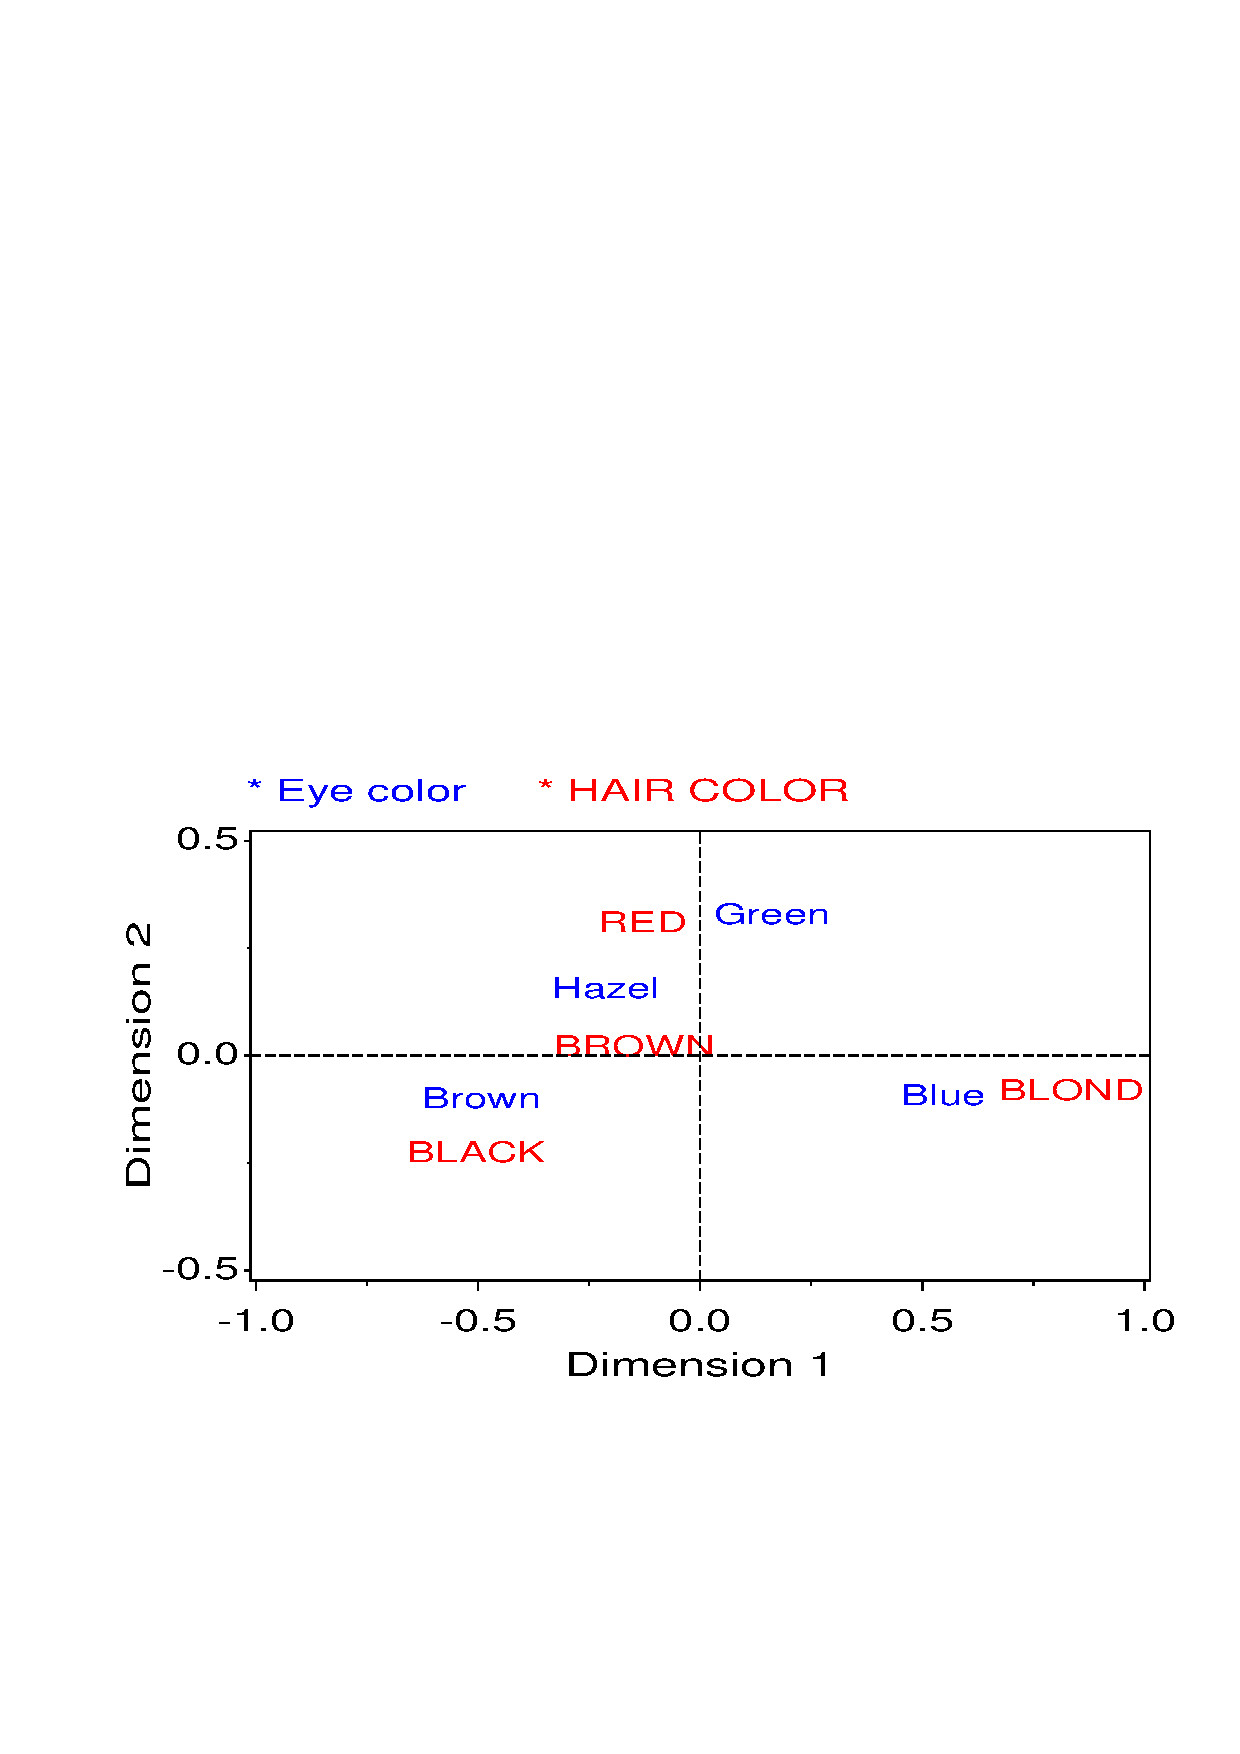
\includegraphics[scale=.7,clip=true]{ch5/fig/corresp3}
  \caption{Correspondence analysis solution for
Hair color, Eye color data}\label{fig:corresp3}
\end{figure}
\ixd{hair-eye color}
\end{Example}

\subsection{The \macro{CORRESP}}\label{sec:ca-camacro}

The steps illustrated in \exref{ex:haireye3} are not difficult, but it is somewhat tedious to do them repeatedly.
The \macro{CORRESP} (documented in \macref{mac:corresp})
is designed to make it easy to produce reasonable plots for \CA\
results.

The \macro{CORRESP}
\begin{itemize}
\item is designed as a simple macro interface to the \proc{CORRESP}.

\item It handles input in either contingency table form
(columns specified by the \mparm{VAR=}{CORRESP}, rows by the
\mparm{ID=}{CORRESP}), or frequency or case form 
(using the \mparm{TABLES=}{CORRESP}).

\item Three-way and larger tables may be analyzed by the ``stacking''
approach to
\mway\ tables described in \secref{sec:ca-multiway}, or by
the MCA approach.

\item Optionally, the macro produces a labeled printer plot and/or
\hires\ graphics plot, with many options for controlling the appearance
of graphics plots.
Axes for \hires\ plots may be equated automatically.
\item An \ODS\ containing the point coordinates and an \ADS\ containing point labels
are produced for further plotting or customization.
\end{itemize}

\begin{Example}[mental1]{Mental impairment and parents' SES}
\citet[p. 289]{Srole-etal:78} give the data below on the mental
health status of a sample of 1660 young New York residents in midtown Manhattan
classified by their parents' socioeconomic status (SES);
see \datref{dat:mental}.
There are five categories of SES and mental health is classified
in the four categories ``well'', ``mild symptom formation'',
``moderate symptom formation'', and ``impaired''.
These data have also been analyzed by many authors, including
\citet[ \S 8.5.2]{Agresti:90},
\citet{Goodman:79}, and
\citet[p. 375]{Haberman:79}.

The statements below read the data in contingency table form with rows identified
by the variable \pname{SES} and column variables \pname{well mild moderate impaired}.
These variables are used in the \verb|%CORRESP| call as the \pname{ID=}
and \pname{VAR=} parameters, respectively.
The graphics output is shown in \figref{fig:correses}.
\begin{figure}[htb]
  \centering
  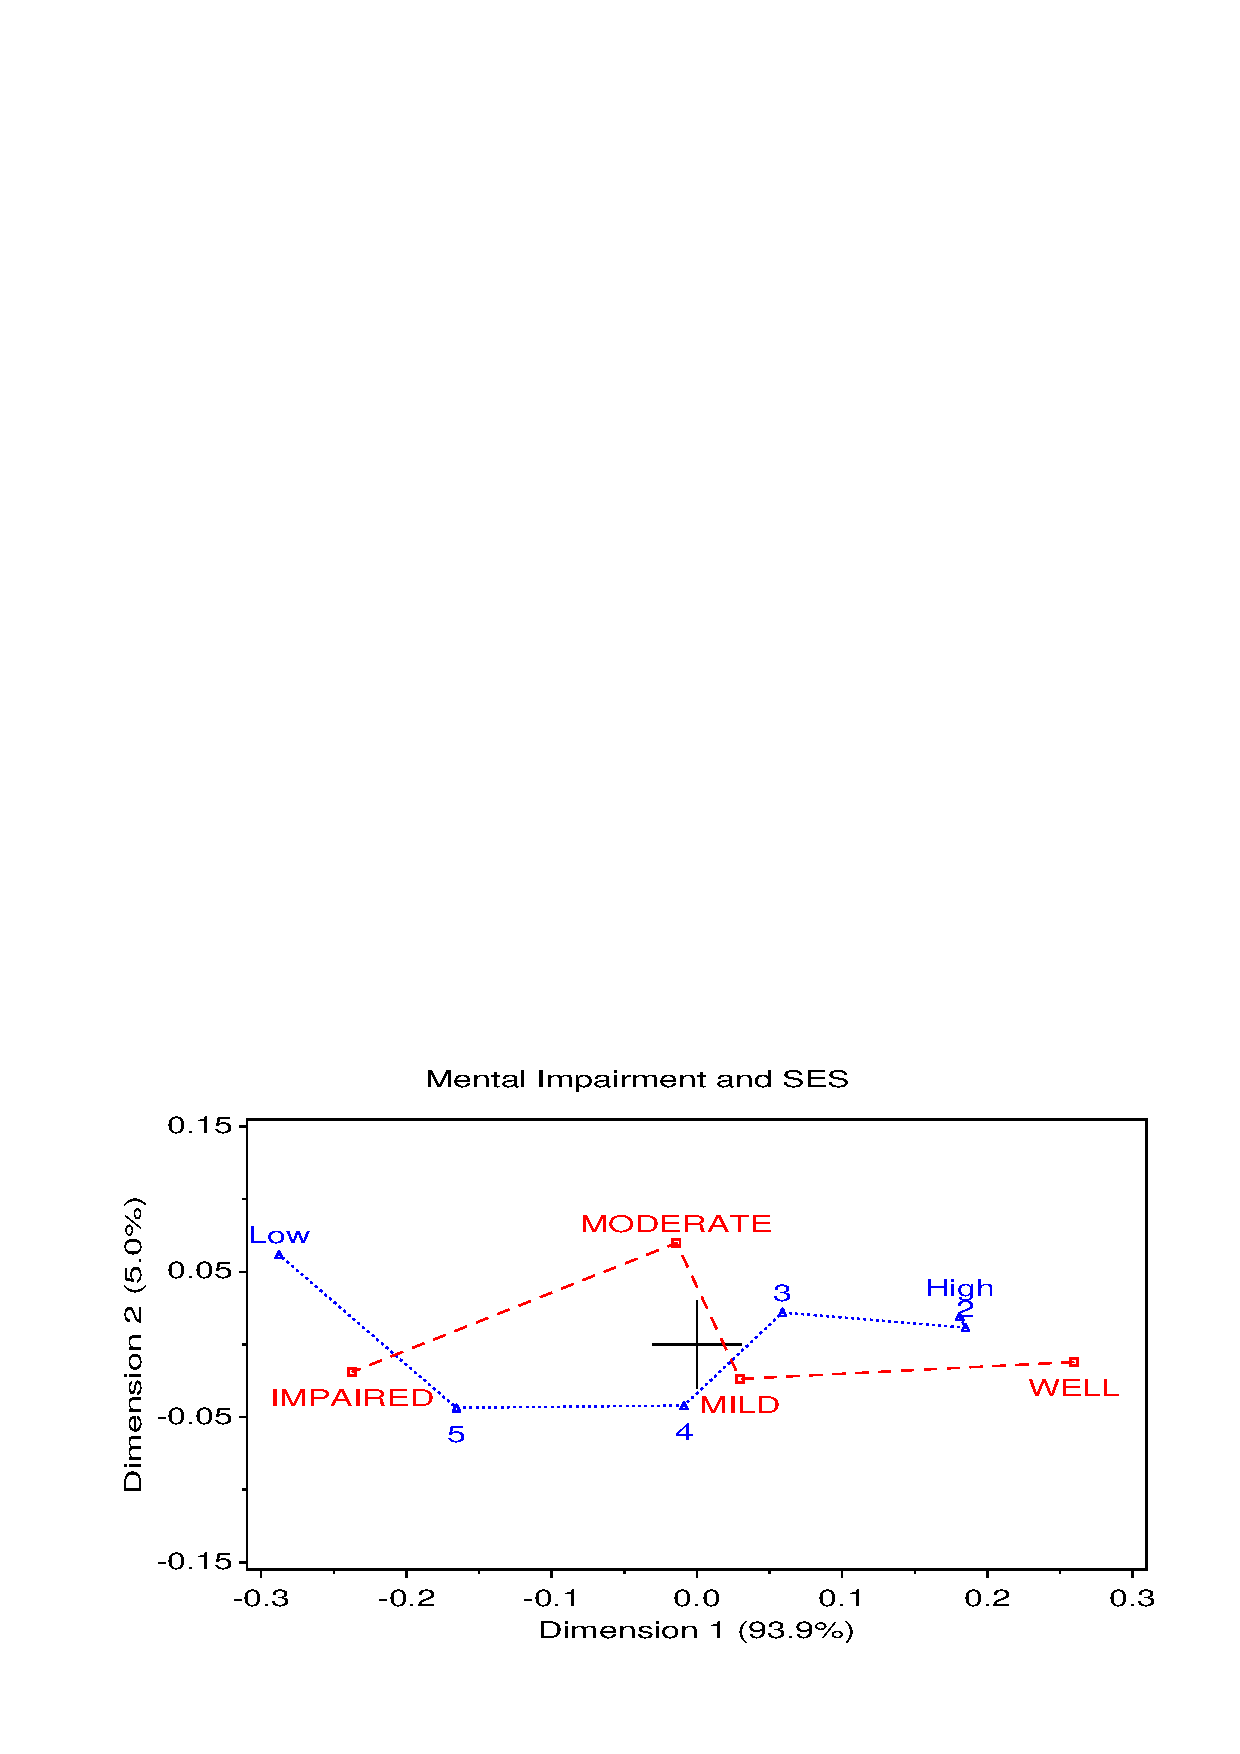
\includegraphics[scale=.8,clip=true]{ch\thechapter/fig/correses}
  \caption{\macro{CORRESP} plot for Mental Health data}\label{fig:correses}
\end{figure}
%% input: /Users/friendly/sasuser/catdata/correses.sas
%% last modified: 25-Jul-99  8:31
\begin{listing}
title h=1.5 lspace=3.8in 'Mental Impairment and SES';
data mental;
   input ses $ well mild moderate impaired;
datalines;
High 64     94     58     46
2    57     94     54     40
3    57    105     65     60
4    72    141     77     94
5    36     97     54     78
Low  21     71     54     71
;
axis1 length=3 in  order=(-.15 to .15 by .10)
      label=(h=1.5 a=90 r=0);
axis2 length=6 in  order=(-.30 to .30 by .10)
      label=(h=1.5) offset=(1);
%corresp (data=mental, id=ses, var=Well Mild Moderate Impaired,
      vaxis=axis1, haxis=axis2, htext=1.3, pos=-, interp=join,
      symbols=triangle square);
\end{listing}

Some of the graphics options for the \macro{CORRESP}
are illustrated by the \pname{htext=} (height of text labels),
\pname{pos=} (position of text labels), \pname{interp=} (point marker interpolation),
and \pname{symbols=} (point symbols) options.
In particular, the option \pname{pos=-} causes the macro to position the text labels
centered above or below the point depending on whether the $y$ position is positive
or negative
(as provided by the \macro{LABEL}; see \macref{mac:label}).

The cross at the origin in \figref{fig:correses} is drawn with equal data units in the
$x$ and $y$ direction, and so serves as a guide to whether the axes
have been equated.  The \pname{LENGTH} and \pname{ORDER} values on the \stmt{AXIS}{GPLOT}s
shown above
were determined by inspection after an initial plot.

We see from the plot that the association between mental health
and parents' SES is almost entirely 1-dimensional, with 94\% of
the \chisq\ ( 45.98, with 15 df) accounted for by Dimension 1.
The diagnostic categories are well-aligned with this dimension and
the two intermediate categories are closer on this dimension than
the extremes, indicating that their profiles differ little.  The
SES categories are also aligned with Dimension 1, and approximately
equally spaced, with the exception of the highest two categories.
Because both row and column categories have the same pattern on
Dimension 1, we may interpret the plot as showing that the profiles
of both variables are ordered, and their relation can be explained
as a positive association between parents' SES and higher mental
health status of children.

From a modeling perspective,  we might ask how strong is the evidence
for the spacing of categories noted above.  For example, we might
ask whether assigning integer scores to the levels of SES and mental
impairment provides a simpler, but satisfactory account of their association.
This question will be explored in a later chapter (see \exref{ex:mental2}).
\end{Example}

%% input: /users/faculty/friendly/sasuser/mosaics/victims.sas
%% last modified: 05-May-98 15:46
\begin{listing}
   *-- rearrange rows/cols by CA dim1;
   keep = \{2 3 1 5 4\};
   table = table[keep,keep];
   lnames = lnames[,keep];
 
   *-- standardize table to equal margins;
   avg = table[,+] / levels[1];
   newtab = repeat(avg,1,5);
   config = \{1 2\};
   call ipf(adjusted, status, levels, newtab, config, table);
   title  = 'Repeat Victimization Data, Adjusted to Equal Margins';
   lab = crime[keep];
   print title, adjusted[r=lab c=lab f=8.2];
   plots = 2;
   run mosaic(levels, adjusted, vnames, lnames, plots, title);

   *-- fit quasi-independence (ignore diagonal cells);
   title  = 'Repeat Victimization Data, Quasi Independence';
   zeros = J(5,5) - I(5);
   run mosaic(levels, adjusted, vnames, lnames, plots, title);
quit;
\end{listing}

\subsection{Quasi-independence and structural zeros}\label{sec:ca-quasi}
\ixon{quasi-independence}
\ixon{structural zeros}
\ixon{zeros!structural}
Incomplete tables can result when particular cells are simply not observed
(sampling zeros, e.g., insufficient data collected) or when some combinations of levels cannot logically occur (structural zeros, e.g., pregnant males).
Alternatively, in some cases we may wish to ignore the data in some cells,
and fit a quasi-independence model to the remaining cells. This is commonly
done with square tables having the same row and column categories,
where the dominant diagonal cells cause a global independence model to fail.

Because CA decomposes departures from independence,
many of these cases can be handled simply by estimating the expected
frequencies which would occur in these cells
if the row and column variables were
independent, and replacing the zero, missing, or dominant observed
frequencies by their expected values.%
\footnote{This does not, however, account properly for the loss in
degrees of freedom, but significance tests in CA are usually not
treated formally.
Indeed, the method would be of little interest for data in which
independence holds.}
More general, iterative procedures are discussed by \citet[\S 8.5]{Greenacre:84}
and by \citet[Ch. 3]{Heijden:87}.

\begin{Example}[victims3]{Repeat victimization}
\exref{ex:victims} also showed a mosaic display 
(\figref{fig:victims3}) for the model of quasi-independence
ignoring the diagonal cells in the repeat victimization data.
The analysis below gives another view of this model.

The elements in the diagonal cells of the \pname{VICTIMS} \Dset\
can be replaced by their expected frequencies under independence
in the following \IML\ step.
\begin{listing}
proc iml;
   use victims;
   read all var _num_  into table[r=crime c=vars];
   read all var {crime} into crime;
   close victims;

   exp = table[,+] * table[+,] / table[+,+];
   table = table + diag(vecdiag(exp - table));

   create victims from table[r=crime c=vars];
   append from table[r=crime c=vars];
\end{listing}
Using the same \verb|%CORRESP| step and plotting steps
as in \exref{ex:victims2} (with a different \stmt{LEGEND}{GPLOT})
gives the 2D plot shown in
\figref{fig:corresp5b}.

%% one figure
\begin{figure}[htb]
  \centering
  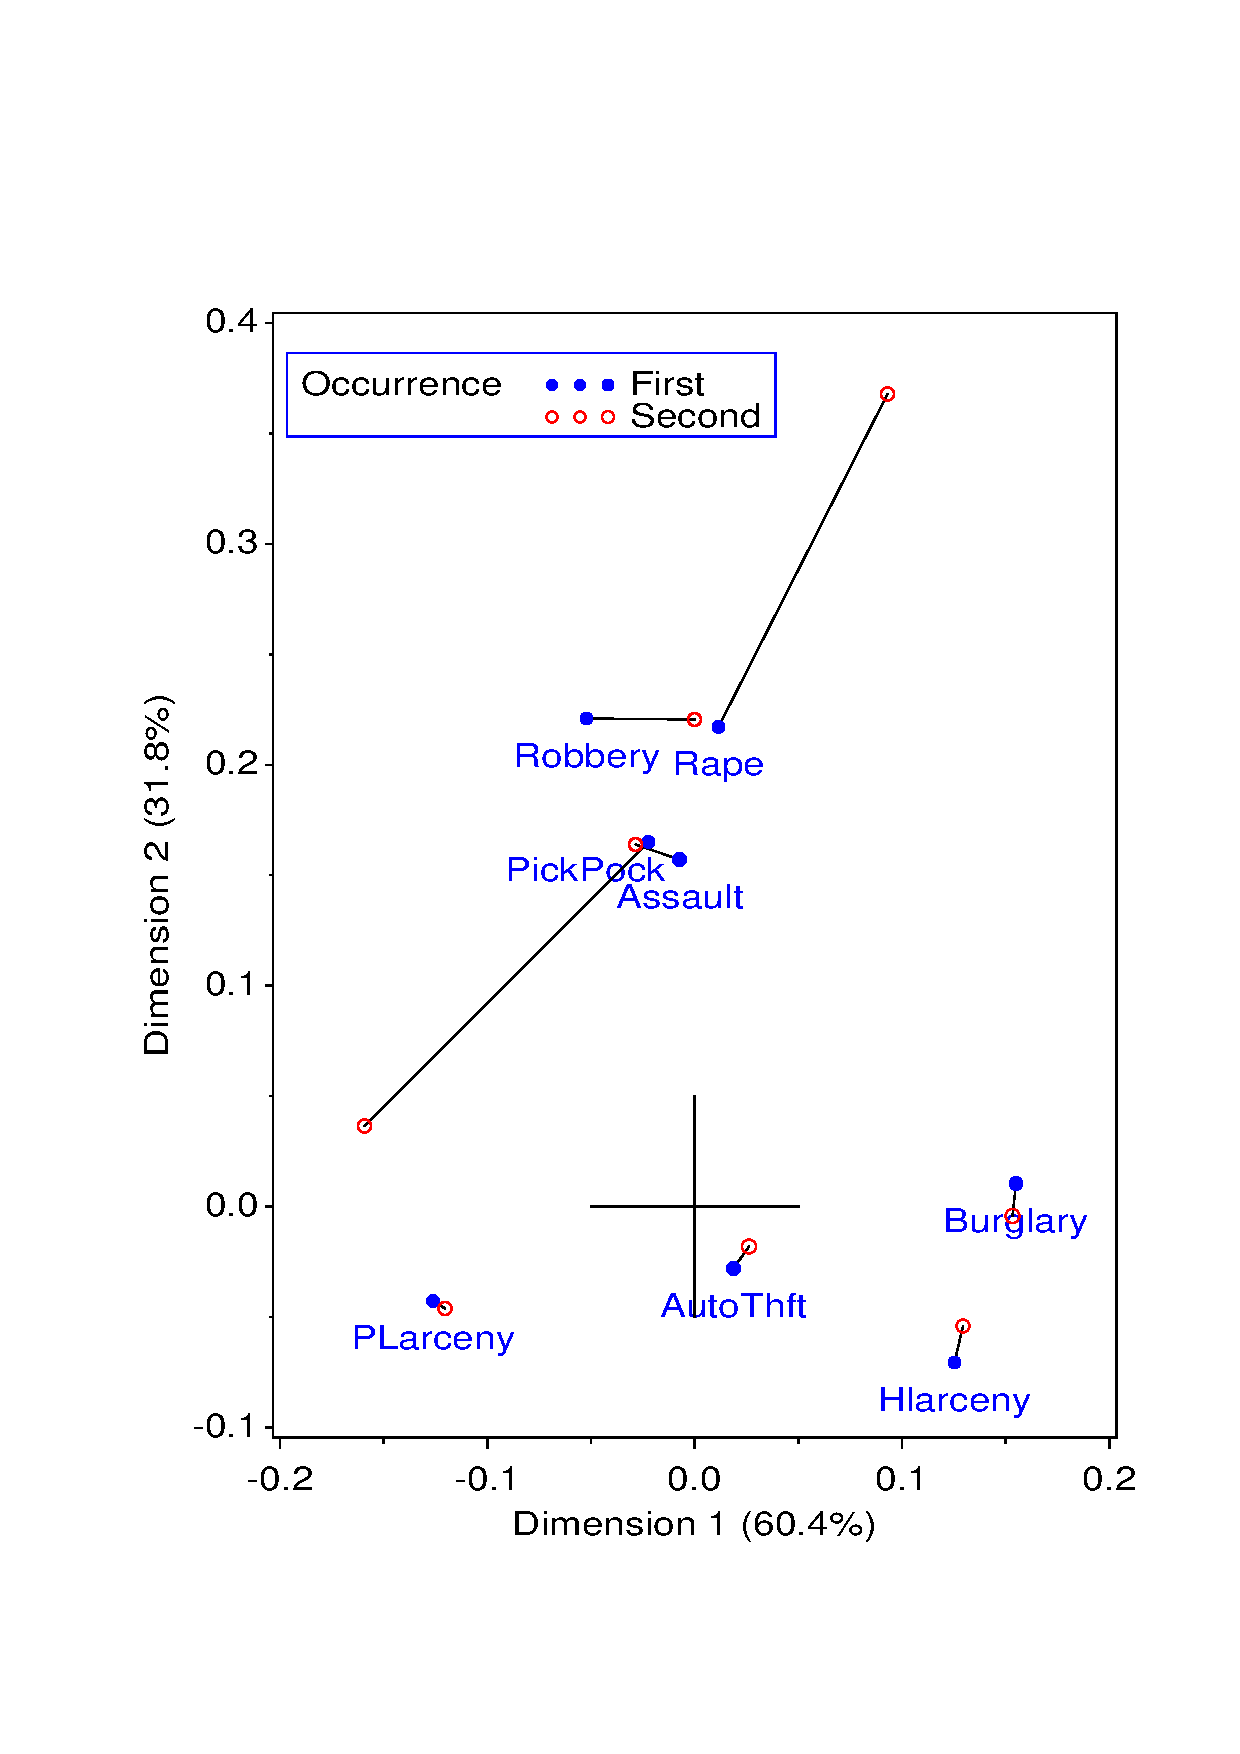
\includegraphics[scale=.6,clip]{ch5/fig/corresp5b}
  \caption[Repeat victimization data, quasi-independence
  model]{2D \CA\ display for repeat victimization data, quasi-independence
  model, ignoring diagonal cells.}%
  \label{fig:corresp5b}
\end{figure}
Note that the 2D solution now accounts for 92\% of the remaining
association, which now concerns only the cells where the crime differs
from first to second occurrence.
For these cells, the differences between first and second incident are
magnified.
\end{Example}
\ixoff{zeros!structural}
\ixoff{structural zeros}
\ixoff{quasi-independence}

\ixoff{correspondence analysis!two-way tables}
\section{Properties of category scores}
This section illustrates several properties of the \CA\
scores through calculation and visualization.

\subsection{Optimal category scores}\label{sec:scores}
The singular values shown in \outref{out:corresp3.1} are the \(\lambda_i\), in Eqn. \eqref{eq:cadij}.  They are also the
(canonical) correlations between the optimally scaled categories.
Thus, if the \pname{DIM1} scores for hair color and eye color are assigned to
the 592 observations in the table, the correlation of these variables
would be 0.4569 --- the largest possible correlation for \emph{any}
assignment of scores.
The \pname{DIM2} scores give a second, orthogonal scaling
of these two categorical variables, whose correlation would be
0.1491.

In this sense, CA scores provide an optimal way of transforming
categorical water into quantitative wine,  hence the name ``optimal
scaling''.

We can illustrate this numerically and visually
as follows. If the row scores on dimension 1 are
in the $r \times 1$ vector $\vec{x}_1$ and the column scores are in the
$c \times 1$ vector $\vec{y}_1$, then these scores can be expanded to
conform with the $r \times c$ table by forming the appropriate outer
product with a unit vector:
\begin{equation*}
 \mat{X}_1 = \vec{x}_1 \: \vec{1}\trans
 \qquad \mbox{and} \qquad
 \mat{Y}_1 = \vec{1} \: \vec{y}_1\trans
 \period
\end{equation*}

The program below uses \IML\ to perform this operation on the \pname{COORD}
\Dset\ and then merges these scores with a reshaped copy of the
\pname{haireye} data.
The resulting \Dset\ is shown in \outref{out:cascores.1}.

The \CA\ scores then serve to quantify the hair color and eye color
categories producing the maximal possible correlations of $(X1, Y1)$ and
$(X2, Y2)$, while all other pairs are uncorrelated.
These correlations are shown in \outref{out:cascores.2}.
A plot of the optimal scores, using cell frequencies as weights
(\figref{fig:cascores}) is developed in the next subsection.
%% input: /users/faculty/friendly/sasuser/catdata/cascores.sas
%% last modified: 29-Jul-98 15:28
\begin{listing}
*-- Attach X, Y values to eye color, hair color and reshape;
proc iml;
   use coord;
   read all var\{dim1 dim2\} where (_type_='VAR') into var[r=eye]; hair=eye;
   read all var\{dim1 dim2\} where (_type_='OBS') into obs[r=eye];
   
   r = nrow(obs);
   c = nrow(var);
   x1 = obs[,1] * j(1, c);
   x2 = obs[,2] * j(1, c);
   y1 = j(r,1)  * t(var[,1]);
   y2 = j(r,1)  * t(var[,2]);
   
   hair = repeat( hair, r, 1);
   eye  = shape(repeat( eye, 1,c),r*c, 1);

   create scores var\{eye hair x1 y1 x2 y2\};
   append;
   quit;

*-- Reshape data to frequency form and merge with scores;
proc transpose data=haireye out=haireye2;
   var BLACK BROWN RED BLOND;
   by eye notsorted;

data haireye2;
   set haireye2;
   rename _name_=hair col1=count;

data scores;
   merge haireye2 scores;

proc print data=scores;
   format x1 x2 y1 y2 7.4;
   id eye hair;

*-- Correlations of scores = singular values;
proc corr data=scores nosimple;
   freq count;
   var x1 x2;
   with y1 y2;   

\end{listing}


\begin{Output}[htb]
\caption{Hair-eye data, DIM1, DIM2 scores assigned to hair-eye categories}\label{out:cascores.1}
\small
\verbatiminput{ch5/out/cascores.1}
\end{Output}
\ixd{hair-eye color}

\begin{Output}[htb]
\caption{Hair-eye data, correlations between X1, X2 and Y1 Y2}\label{out:cascores.2}
\small
\verbatiminput{ch5/out/cascores.2}
\end{Output}
\ixd{hair-eye color}

\subsection{Simultaneous linear regressions}
The correlations among the \CA\ scores have yet another interpretation which gave
rise to the first algebraic derivation of the technique
\citep{Hirschfeld:35} and which today provides an important concept in the
\citet{Gifi:90} system of homogeneity analysis.

Consider an arbitrary assignment of scores $X1$ ($Y1$) to the hair color
(eye color) categories, for example $X1$ ($Y1$) = 1, 2, 3, 4 for the
categories in alphabetical order.
Instead of plotting these scores along a dimension as in \figref{fig:corresp3}, we plot $Y1$ against $X1$ for all $n = 592$
cases and show the frequency at each discrete point by the area of
a bubble symbol, as in \figref{fig:cascore0}.

\begin{figure}[htb]
  \centering
  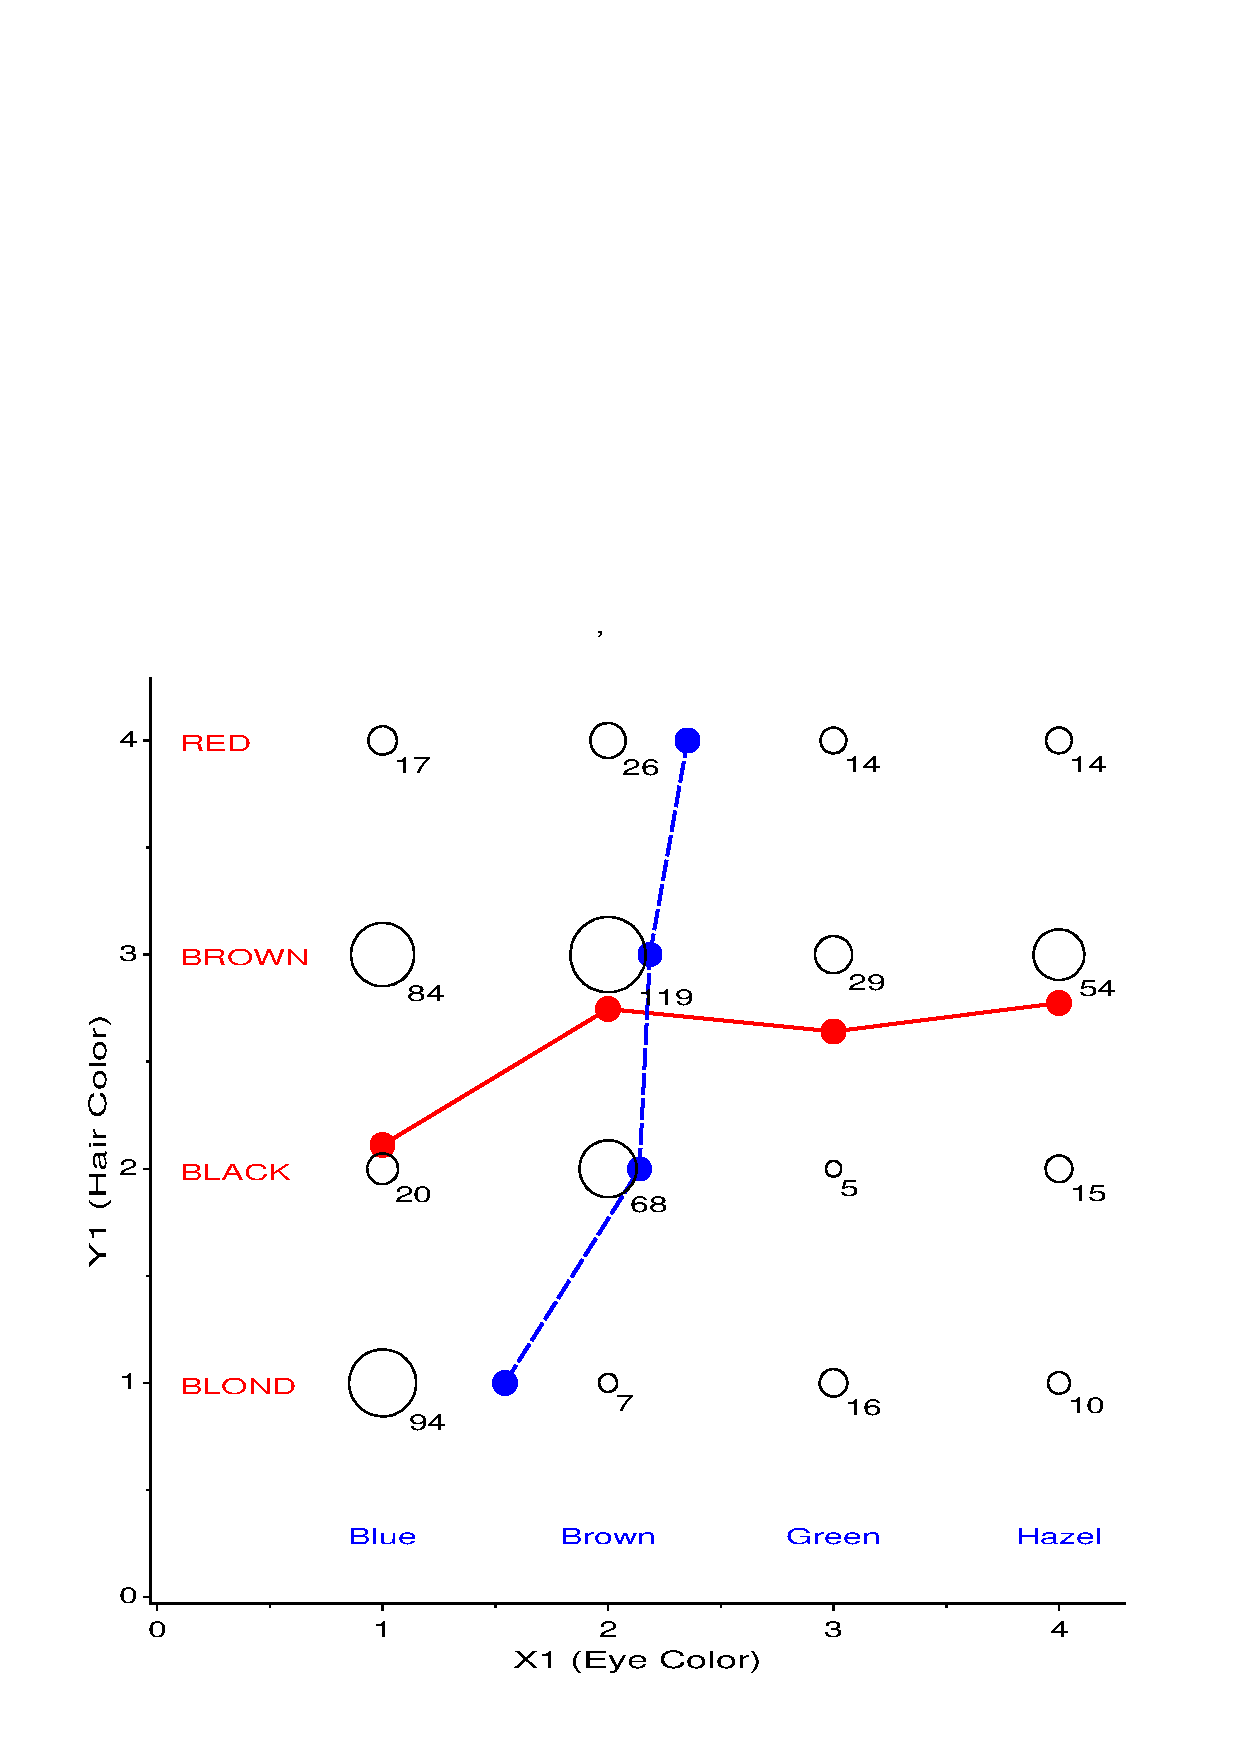
\includegraphics[scale=.6,clip]{ch5/fig/cascore0}
  \caption[Plot of arbitrary scores for the row and column categories]{Plot of arbitrary scores for the row and column categories.
The bubble symbols and numbers show the frequency at each point.
The red points (solid line) show the means of $Y1\given X1$; blue points (dashed line) show the means of $X1\given Y1$.}\label{fig:cascore0}
\end{figure}

If we carried out a least squares regression of  $Y1$ on $X1$,
this would be equivalent to finding the weighted mean of  $Y1$ for each value of $X1$ and fitting a straight line to these means.
Similarly, we could fit a regression of $X1$ on $Y1$,  which would be
determined by the weighted means of $X1$ for each $Y1$.
For the arbitrary scores, the conditional means of $Y1\given X1$
have a nonlinear relation to $X1$, and the same is true for the
inverse regression of $X1\given Y1$, as we see in \figref{fig:cascore0}.
The question posed by \citet{Hirschfeld:35} was this:
Can we find scores $\vec{a}$ and $\vec{b}$ for the row and column
variables such that \emph{both} regressions are linear?

The answer is ``Yes!''; indeed there is one solution for each pair of
\CA\ scores, $\vec{a}_i$ and $\vec{b}_i$, associated with the singular value $\lambda_i$.
For a given set of scores, $\vec{a}_i$ and $\vec{b}_i$, the weighted means
of the columns are
\(\mat{D}_c^{-1} \mat{P} \trans \vec{a}_i \), and the linear regression on
$\vec{b}_i$ has intercept 0 and slope $\lambda_i$,
\begin{equation*}%\label{eq:calin1}
(\mat{D}_c^{-1} \mat{P} \trans) \vec{a}_i = \lambda_i \vec{b}_i
\end{equation*}
Similarly, the inverse regression on $\vec{a}_i$ has intercept 0 and slope $1/\lambda_i$
\begin{equation*}%\label{eq:calin2}
(\mat{D}_r^{-1} \mat{P}) \vec{b}_i = (1/\lambda_i) \vec{a}_i
\end{equation*}
The choice of the scores associated with the largest singular value,
$\lambda_1$, makes the slope (equivalently, the correlation) of the
regression of $Y1$ on $X1$ as large as possible.
Moreover, this choice makes the angle between the two regression lines
as small as possible, i.e., the regressions are most collinear
\citep{Greenacre:84}.
So, instead of complex, nonlinear relations between the scaled
hair color and eye color variables using arbitrary scores (\figref{fig:cascore0}),
we arrive at simple, linear relations by use of a nonlinear
transformation of the arbitrary scores.

We can show these regressions for the first \CA\ dimension
in the following program steps, which continue from those
shown in \secref{sec:scores}.
Most of the program steps are concerned with finding the means
of $Y1\given X1$ and $X1\given Y1$, and annotating them on the
plot, together with the category labels and the regression line.
The plot with both regression lines is shown in \figref{fig:cascores}.
\begin{figure}[htb]
  \centering
  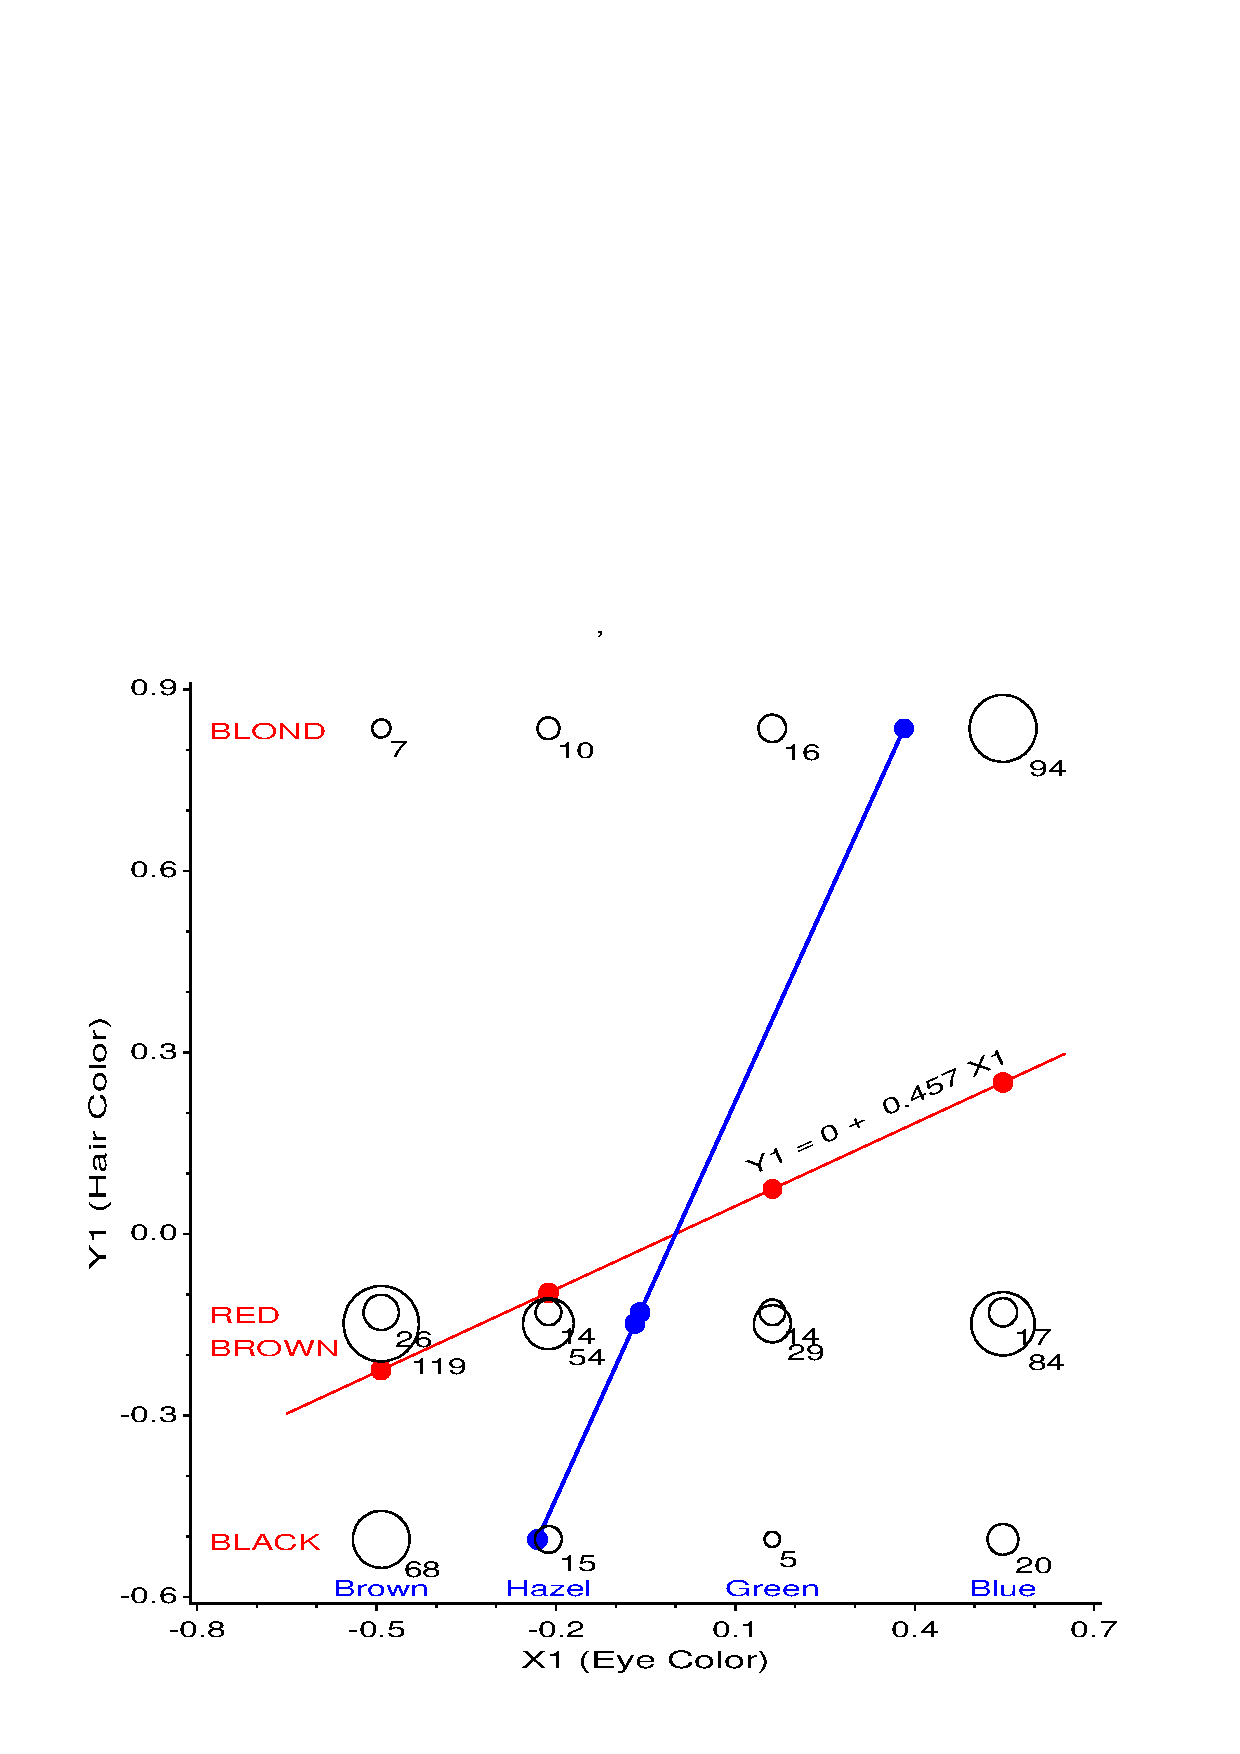
\includegraphics[scale=.6,clip]{ch5/fig/cascores}
  \caption[Simultaneous linear regressions of \CA\ scores for dimension 1]{Simultaneous linear regressions of \CA\ scores for dimension 1.  Using the optimal scores makes both regressions linear; choosing the scores associated with the largest singular value makes the two regressions most collinear.}\label{fig:cascores}
\end{figure}
%% input: /users/faculty/friendly/sasuser/catdata/cascores.sas
%% last modified: 04-Aug-98 13:31
\begin{listing}
*-- Annotate the row and column means;
proc means data=scores nway noprint;
   var y1;
   class x1;
   freq count;
   output out=ymeans mean=y1bar;
data ymeans;
   set ymeans;
   retain xsys  ysys '2' size 2;
   x = x1; y = y1bar;
   function = 'symbol'; text='dot'; color='red';  output;

proc means data=scores nway noprint;
   var x1;
   class y1;
   freq count;
   output out=xmeans mean=x1bar;
data xmeans;
   set xmeans;
   retain xsys  ysys '2' size 2 line 4;
   x = x1bar; y = y1;
   function = 'symbol'; text='dot'; color='blue';  output;
   if _n_=1 then function='move';
      else function='draw';
   output;

*-- Annotate the row and column labels;
data label1;
   set scores(keep=eye hair x1 y1);
   where eye='Brown';
   retain xsys ysys '2' color 'red    ' function 'label   ';
   if hair='BROWN' then position='9';
      else position='6';
   x = -.78; y = y1; text = hair;
data label2;
   set scores(keep=eye hair x1 y1);
   where hair='BLACK';
   retain xsys ysys '2' position '5' color 'blue' function 'label   ';
   x = x1; y = -.58; text = eye;

*-- Get slope and intercept of (weighted) regression line;
proc reg data=scores outest=parms noprint;
   model y1 = x1;
   weight count;

data line;
   set parms (keep=x1 intercep);
   drop x1 intercep;
   length text $20;
   
   *-- Draw (weighted) regression line;
   xsys='2'; ysys='2'; color='red   ';
   x=-0.65; y = intercep + x1 * x; function='MOVE    '; output;
   x= 0.65; y = intercep + x1 * x; function='DRAW    '; output;
   x= 0.35; y = intercep + x1 * x; function='LABEL   '; color='black';
   angle = atan(x1) * (45/atan(1)); position='2';
   text = 'Y1 = 0 + ' || put(x1,6.3) || ' X1';  output;
   
*-- Combine the annotate data sets;
data labels;
   length text $20;
   set label1 label2 line ymeans xmeans;

proc gplot data=scores;
   bubble y1 * x1 = count / 
      blabel bsize=8 bscale=area
      vaxis=axis1 haxis=axis2 hm=2 vm=2 anno=labels;
   axis1 order=(-.6 to .9 by .3) label=(h=1.8 a=90 'Y1 (Hair Color)');
   axis2 order=(-.8 to .7 by .3) label=(h=1.8      'X1 (Eye Color)');
   \end{listing}

Note that the slope of the line for $Y1\given X1$ in \figref{fig:cascores} is 0.457, the largest singular value and the largest canonical correlation.
If we were to repeat these steps using the \CA\ scores $X2$ and $Y2$
on dimension 2, we would find another pair of linear regressions, with
a slope of 0.149 for $Y2\given X2$, the second singular value.

